\section{Flow-Path Planning}
\label{sec:flow_paths}

After completing the architectural synthesis above, a biochip architecture with exact device locations as well as optimized channel connections is generated. In this subsection, the proposed flow-path planning for moving fluids will be discussed in detail. Our goal is to implement all the fluid transportation/caching tasks without any conflict, so that the bioassay can be completed within a short time. Moreover, extra resources such as ports and channel segments introduced to the biochip can also be minimized during the flow-path planning.

\subsection{Flow-Path Planning on A Given Biochip Architecture}
\label{sec:constructing_paths_given}

\begin{figure}[t]
    \centering
    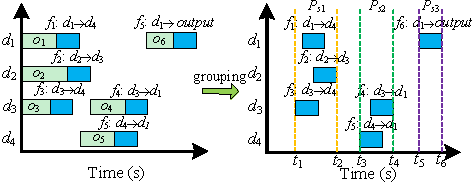
\includegraphics[width=1.0\linewidth]{Visio/task_division.pdf}
  \caption{Illustration of transportation-task grouping during flow-path planning.}
      \label{fig:concurrent_set}
% \vspace{-0.5cm}
\end{figure}

As discussed previously, transportation tasks may be performed concurrently in a scheduling scheme. To avoid conflict among them, the flow paths used for these tasks should avoid to share any on-chip resource, and this therefore requires that all the parallel tasks should be identified from the scheduling before implementing the real flow-path planning.

Accordingly, in the proposed method, we adopt an efficient sweepline algorithm \cite{lane1979generalized} to divide all the transportation tasks in a scheduling into multiple groups, while ensuring that tasks in the same group will be performed in parallel. During the sweeping, a vertical line is used to scan the entire scheduling diagram from left to right along the time axis. Moreover, we maintain an active task group $P_{s}$ to record all the parallel transportation tasks at the currently scanned time interval. Each time when the sweeping line encounters a transportation task $f_r$, if $P_s=\emptyset$ or $f_r$ overlaps with at least one task in $P_s$ in their execution time, $f_r$ will be added to $P_s$. Otherwise, $P_s$ will be stored temporarily and the scanning will be continued using a new active task group with $f_r$ as its first element. As the result of the whole scanning process, several task groups can be generated and each of them consists of a set of parallel transportation tasks. For example, \figname~\ref{fig:concurrent_set} shows the scheduling scheme of a bioassay, where a total of six transportation tasks ($f_1$--$f_6$) are scheduled to complete the execution of specified operations. After implementing the sweepline algorithm discussed above, the transportation tasks in \figname~\ref{fig:concurrent_set} are divided into the following three groups:

\begin{itemize}
\item
$P_{s1}$: \{task$|f_1,f_2,f_3$\}, (time interval, $t_1\to t_2$)
\item
$P_{s2}$: \{task$|f_4,f_5$\}, (time interval, $t_3\to t_4$)
\item
$P_{s3}$: \{task$|f_6$\}, (time interval, $t_5\to t_6$)
\end{itemize}

Since transportation conflicts can only occur among parallel tasks, this enables us to deal with the flow-path planning problem according to the task grouping result above. In other words, a flow-path planning solution without transportation conflicts can be obtained by sequentially constructing flow paths for the tasks in each group. Accordingly, based on the connection grid modelled in \figname~\ref{fig:grid_model} as well as the chip architecture generated in Section~\ref{sec:channel_storage_synthesis}, we formulate the flow-path planning problem into an ILP model to efficiently find an optimized solution.

Given a task group $P_s$ obtained by the sweepline algorithm, our goal is to find an optimized flow path for each transportation task in $P_s$, while ensuring that these paths do not share any on-chip resource. More specifically, for a task $f_r\in P_s$ with $d_i$ and $d_j$ as its source and target devices, assume that $d_i$ and $d_j$ are assigned to nodes $n_i$ and $n_j$ in the connection grid. Since the flow path of $f_r$ is required to start with a pump and ends with a waste port while it passes through both $d_i$ and $d_j$, we use a 0-1 variable $u^r_{n_k}$  to represent whether a node $n_k$ is on the flow path of $f_r$. Thus we derive the following constraints
\begin{align}
& \sum_{n_k\in N_p}u^r_{n_k} = 1,\; \sum_{n_k\in N_w}u^r_{n_k} = 1 \label{eq:flow_node_1} \\
&\;  u^r_{n_i} = 1,\; u^r_{n_j} = 1\label{eq:flow_node_2}
\end{align}
where $N_p$ and $N_w$ are nodes occupied by pump ports and waste ports, respectively. Note that the positions of these ports are scattered to some empty nodes in the connection grid.

On the other hand, if task $f_r$ transports the resulting fluid of device $d_i$ to a channel segment bound to edge $e_j$ for temporary caching, constraint \text{(\ref{eq:flow_node_2})} can be reformulated as
\begin{align}
&  u^r_{n_i} = 1,\; u^r_{e_j} = 1\label{eq:flow_node_3}
\end{align}
where $u^r_{e_j}$ is a 0-1 variable representing whether an edge $e_j$ is on the flow path of $f_r$.

In addition, channel segments on the chip, in other words edges on the grid, used for connecting the devices and ports on the flow path of $f_r$ need to be determined. Note that at the pump port or the waste port, only one of the four adjacent edges can be covered in the path. At each other device on the path, exactly two adjacent edges are covered by the path. Accordingly, the flow path $f_r$ can be computed with the following constraints
\begin{align}\label{eq:continuous}
&  \sum_{e_j\in E_{n_p}}u^r_{e_j} - (1-u^r_{n_p})M \leq 1,\; \forall n_p\in N_p\\
&  \sum_{e_j\in E_{n_p}}u^r_{e_j} + (1-u^r_{n_p})M \geq 1,\; \forall n_p\in N_p\\
&  \sum_{e_j\in E_{n_w}}u^r_{e_j} - (1-u^r_{n_w})M \leq 1,\; \forall n_w\in N_w\\
&  \sum_{e_j\in E_{n_w}}u^r_{e_j} + (1-u^r_{n_w})M \geq 1,\; \forall n_w\in N_w\\
&  \sum_{e_j\in E_{n_k}}u^r_{e_j} - (1-u^r_{n_k})M \leq 2,\; \forall n_k\in N_d\backslash \{N_p,N_w\}\\
&  \sum_{e_j\in E_{n_k}}u^r_{e_j} + (1-u^r_{n_k})M \geq 2,\; \forall n_k\in N_d\backslash \{N_p,N_w\}\label{eq:continuous_last}
\end{align}
where $E_{n_p}$, $E_{n_w}$, and $E_{n_k}$ are the sets of edges adjacent to the nodes $n_p$, $n_w$, and $n_k$, respectively. $N_d$ represents all the nodes occupied by devices in the connection grid. $M$ is a very large constant to transform the formulas above into linear constraints.

Another issue that needs to be considered is that the flow path of $f_r$ should bypass the devices used for other on-going operations as well as the channel segments used for fluid caching. These constraints can be formulated as
\begin{align}
&   u^r_{n_k} = 0,\; \forall n_k\in N_b \label{eq:bypass0} \\
&   u^r_{e_j} = 0,\; \forall e_j\in E_b \label{eq:bypass}
\end{align}
where $N_b$ is the set of nodes occupied by other active devices and $E_b$ is the set of edges occupied by  channels for caching.

Finally, to avoid transportation conflict between flow paths, for any transportation task $f_s\in P_s$, the flow paths of $f_s$ should not share any node on the chip with that of $f_r$, leading to the following constraint
\begin{align}
& u^r_{n_k} + u^s_{n_k} \leq 1,\; \forall n_k\in N \label{eq:nonconflict}
\end{align}
where $N$ is the set of nodes in the connection grid.

In practice, the transportation time of fluids as well as the pressure used for driving the movement of fluids are strongly affected by to the length of flow paths \cite{hu2015fault}. Hence, this length should be minimized and the exact flow paths for all the transportation tasks can be computed by solving the following optimization problem
\begin{align}\label{eq:ILP_flow_paths}
\text{minimize} &\; \sum_{f_r\in F_t} \sum_{e_j\in E_c} u^r_{e_j} \\\label{eq:ILP_flow_paths_last}
\text{subject to} & \;
\text{(\ref{eq:flow_node_1})--(\ref{eq:nonconflict})}
\end{align}
where $F_t$ is the set of transportation tasks in the scheduling scheme and $E_c$ is the set of edges occupied by channel segments in the connection graph.

\subsection{Deadlock Removal}\label{sec:res_storage_deadlock}

As discussed in Section~\ref{sec:flow_path_chan}, deadlock may occur in a distributed channel-storage system due to the dual functions of flow channels, and this may make the optimization problem defined in \text{(\ref{eq:ILP_flow_paths})--(\ref{eq:ILP_flow_paths_last})} unsolvable. To address the deadlock problem without introducing extra resources to the biochip architecture, fluids cached in those blocked paths need to be moved to other unused channel segments. To this end, we use a 0-1 variable $m_j$ to indicate whether the fluid cached in edge $e_j$ needs to be moved away such that the current deadlock can be eliminated. Accordingly, constraint \text{(\ref{eq:bypass})} can be reformulated as
\begin{align}\label{eq:bypass_move}
   u^r_{e_j} - m_i \leq 0,\; \forall e_j\in E_b.
\end{align}

Moreover, since moving fluids from a channel segment to another can lead to extra cost such as delay of bioassay, the number of movement operations needs to be minimized. Accordingly, the optimization problem defined in \text{(\ref{eq:ILP_flow_paths})}--\text{(\ref{eq:ILP_flow_paths_last})} can be reformulated as
\begin{align}\label{eq:ILP_flow_paths_deadlock}
\text{minimize} & \quad \sum_{f_r\in F_t} \sum_{e_j\in E_c} u^r_{e_j}
+ \sum_{e_j \in E_b} P_f * m_j \\\label{eq:ILP_flow_paths_deadlock_last}
\text{subject to} & \;
\text{(\ref{eq:flow_node_1})--(\ref{eq:bypass0}),\;(\ref{eq:nonconflict}),\;(\ref{eq:bypass_move})}
\end{align}
where the penalty factor $P_f$ is a large constant to punish the movement of cached fluids.

After solving the ILP formulation above, fluids that need to be moved away are known. In other words, if a 0-1 variable $m_j$ is set to 1 in the ILP solution, the corresponding fluid cached in channel segment $e_j$ should be removed so that the deadlock can be eliminated. Moreover, since the flow path for each transportation task has already been determined after solving the ILP formulation, new location for caching the removed fluid can be determined by selecting an unused channel segment without introducing new deadlock. Note that the flow path for transporting the removed fluid can also be constructed using the ILP constraints defined in \text{(\ref{eq:flow_node_1})--(\ref{eq:nonconflict})}.


\subsection{Conflict Elimination -- Scheduling Adjustment}\label{sec:ILP_flow_paths}

On the other hand, transportation conflict is another factor that may render the path-planning formulation in \text{(\ref{eq:ILP_flow_paths})--(\ref{eq:ILP_flow_paths_last})} unsolvable. Accordingly, in Section~\ref{sec:flow_path_chan}, two conflict elimination strategies, i.e., scheduling adjustment and architecture adjustment, are proposed to solve this problem.

\begin{figure}[t]
    \centering
	 \subfloat[]{
       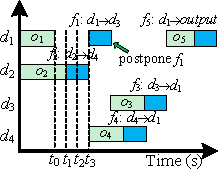
\includegraphics[width=0.48\linewidth]{Visio/postpone_cmp2.pdf}}
    \label{ta}
	\subfloat[]{
        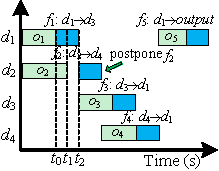
\includegraphics[width=0.48\linewidth]{Visio/postpone_cmp1.pdf}}
    \label{tb}
	  \caption{Comparison on different scheduling-adjustment schemes. (a) Postpone the execution of task $f_1$. (b) Postpone the execution of task $f_2$. }
	  \label{fig:adjusment_choice}
%\vspace{-0.5cm}
\end{figure}

As illustrated in Fig.~\ref{fig:strategy}, the core idea of scheduling adjustment is to postpone the execution of some transportation tasks, so that those conflicting tasks do not overlap in their execution time. Since postponing a transportation task might trigger a chain reaction such that the execution of the complete bioassay is prolonged, choosing an appropriate postponing scheme with minimized overall time extension is crucial to the whole flow-path planning. For example, Fig.~\ref{fig:adjusment_choice} shows two postponing schemes for solving the transportation conflict in Fig.~\ref{fig:motivation}. In Fig.~\ref{fig:adjusment_choice}(a), the starting time of task $f_1$ is postponed from $t_0$ to $t_3$. Since the result of operation $o_1$ is directly related to the execution of both $o_3$ and $o_5$, this leads to a $t_3-t_0$ time extension for the complete bioassay. However, in Fig.~\ref{fig:adjusment_choice}(b), the starting time of $f_2$ is postponed from $t_1$ to $t_2$ and the time extension introduced to the bioassay is only $t_2-t_1$. Although both schemes can eliminate the current transportation conflict, the goal of scheduling adjustment is to find a solution with minimized extra time extension such as in Fig.~\ref{fig:adjusment_choice}(b) .

To realize the scheduling adjustment, we formulate the postponing schemes of transportation tasks as well as the corresponding scheduling results into an ILP model. Assume that $C$ is the set of all feasible postponing schemes, we use a 0-1 variable $c_j$ to represent whether the $j$-th scheme is select to eliminate a transportation conflict. Accordingly, constraint \text{(\ref{eq:nonconflict})} can be reformulated as
\begin{align}
& u^r_{n_k} + u^s_{n_k} + c_j \leq 2, \; \forall n_k\in N, \; \forall c_j\in C \label{eq:postpone1} \\
& \sum_{c_j\in C}c_j = 1 \label{eq:postpone2}
\end{align}
where $p_r$ and $p_s$ are two transforation tasks that overlap in their execution time in scheme $c_j$.

Moreover, to minimize the execution time of the complete bioassay, we adopt the well-known list scheduling algorithm \cite{lawler1993sequencing} to compute the extra extension of execution time introduced by a postponing scheme, and incorporate the corresponding result into our objective function. Accordingly, the optimization problem defined in \text{(\ref{eq:ILP_flow_paths_deadlock})}--\text{(\ref{eq:ILP_flow_paths_deadlock_last})} can be further reformulated as
\begin{align}\label{eq:ILP_flow_paths_deadlock_postpone}
\text{minimize} & \quad \sum_{f_r\in F_t} \sum_{e_j\in E_c} u^r_{e_j}
+ \sum_{e_j \in E_b} P_f * m_j + \sum_{c_j \in C} d_j * c_j \\\label{eq:ILP_flow_paths_deadlock_postpone_last}
 \begin{split}
\text{subject to} & \quad
\text{(\ref{eq:flow_node_1})--(\ref{eq:bypass0}),\;(\ref{eq:bypass_move}),\;(\ref{eq:postpone1})--(\ref{eq:postpone2})}
 \end{split}
\end{align}
where $d_j$ is the extra extension of execution time  introduced by the postponing scheme $c_j$.

\subsection{Conflict Elimination -- Architecture Adjustment}\label{sec:GA}

When biochips are used for large-scale biochemical analysis, a large number of operations need to be executed with limited resources in parallel. Particularly in a distributed channel-storage architecture, a large amount of intermediate fluids needs to be cached in flow channels temporarily and this further aggravates the conflicts among transportation tasks, making the ILP model formulated in \text{(\ref{eq:ILP_flow_paths_deadlock_postpone})}--\text{(\ref{eq:ILP_flow_paths_deadlock_postpone_last})} very difficult to solve. Moreover, the completion of bioassays may also be prolonged severely. Accordingly, in this subsection, we implement the architecture adjustment method proposed in Section~\ref{sec:flow_path_chan} by introducing more resources, such as channel segments, pumps, and waste ports, to the chip architecture, so that the large-scale transportation conflicts discussed above can be solved effectively.

To generate a new biochip architecture with minimized extra resources, we apply the heuristic optimization method Genetic Algorithm, which is first introduced by John Holland in 1975 \cite{mitchell1998introduction}. It is developed based on the concept of Charles Darwin's theory of natural evolution, and has been found to be robust in solving complex engineering and scientific optimization problems.

In the proposed method, a population of candidate solutions, also referred to as chromosomes, is randomly initialized in the whole solution space. The encoding of each chromosome is represented in binary as strings of 0s and 1s. All the chromosomes are then evolved by iteratively updating their encodings using the genetic operators such as mutation and crossover, with the population in each iteration called a generation. In each generation, a fitness value of each chromosome is computed using an evaluation function to assess its solution quality. Finally, the algorithm terminates when a satisfactory fitness level is reached for the population.

Since each chromosome represents an augmented biochip architecture with new introduced resources, its corresponding encoding should include the following information: 1) the locations of newly introduced resources like pumps and waste ports and 2) the locations of newly introduced channel segments. Accordingly, we employ a two-dimensional 0-1 vector $\vec{X} = [\vec{x}^{d}, \vec{x}^{c}]$ to encode a chromosome, where vector $\vec{x}^{d}= [x^d_0,x^d_1,...,x^d_m]$ is used to denote the locations of new resources in the connection grid, which can be defined as
\begin{equation}
  x^d_i =
  \begin{cases}
    1 & \text{if node $n_i$ is occupied by a new resource}\\
    0 & \text{otherwise.}
  \end{cases}
\end{equation}
Vector $\vec{x}^{c} = [x^c_0,x^c_1,...,x^c_n]$ is used to indicate the locations of new channel segments in the connection grid, which can be defined as
\begin{equation}
  x^c_j =
  \begin{cases}
    1 & \text{if edge $e_j$ is assigned to a new channel segment}\\
    0 & \text{otherwise.}
  \end{cases}
\end{equation}

In addition, the fitness of a chromosome is evaluated by three criteria during the evolution of population:
1) if the biochip architecture represented by a chromosome is invalid, in other words, if we still cannot find a feasible flow-path planning solution on the new chip, the fitness of this chromosome is set to $-\infty$, meaning that the newly introduced resources still cannot eliminate all the transportation conflicts, 2) if flow paths for all the transportation tasks can be constructed on the new chip architecture without any conflict, the algorithm tends to select the chromosome that leads to shorter execution time of the bioassay, and 3) our method tends to select the chromosome with minimized extra resources. Accordingly, the evaluation function used in the proposed algorithm can be formulated as
\begin{equation}\label{eq:fitness}
  F(X_i) =
  \begin{cases}
    -\infty & \text{if $X_i$ is invalid}\\
    C_1-C_2\times N_d-C_3\times T_e & \text{otherwise}
  \end{cases}
\end{equation}
where $C_1$, $C_2$, and $C_3$ are three constants, $N_d$ represents the number of extra resources introduced to the chip, and $T_e$ represents the execution time of the bioassay.

The detailed steps of the proposed architecture adjustment method can be summarized as follows:
\begin{enumerate}
  \item
  Based on the previously generated biochip architecture in the connection grid, chromosomes are initialized by randomly introducing new resources as well as channel segments to the chip. These chromosomes form the first generation of the population.

  \item \label{item:iteration_begin}
  For each chromosome $X_i$ in the population, the proposed flow-path planning method is employed to evaluate the biochip architecture represented by $X_i$ and generate a fitness value $F(X_i)$ according to (\ref{eq:fitness}).

  \item
  All the chromosomes are sorted in non-increasing order according to their fitness values, and the first half of the population is then selected as the parent of next generation.

  \item \label{item:new_gen}
  Genetic operators including mutation and crossover are applied to the selected chromosomes to generate new chip architectures. Mutation operation generates a new chromosome by reversing the values of some randomly selected encoding positions on a parent chromosome. Crossover operation exchanges information of some encoding positions between two parent chromosomes. Both the parent and child chromosomes form the next generation of population.

  \item
  Step (2) to (4) are executed repeatedly  until the maximum allowed number of iterations is reached. The biochip architecture represented by the chromosome with the best fitness value is then selected as the final solution.
\end{enumerate}

\begin{table*}[t] 
\footnotesize
\centering
\renewcommand{\tabcolsep}{7.35pt}
\renewcommand{\arraystretch}{1}
\caption{Results of Test Pattern Generation with Single Pressure Source and Single Pressure Sensor}
\label{tb_test}
\begin{tabular}{cr r ccccccc r ccccccc} \hlinewd{0.7pt}
\multicolumn{2}{c}{FPVA} &
\multicolumn{1}{c}{} &
\multicolumn{7}{c}{Direct Approach} &
\multicolumn{1}{c}{} &
\multicolumn{7}{c}{Loop Acceleration} \\
\cline {1-2}\cline {4-10}\cline {12-18} 
\multicolumn{1}{c}{Dimension} &
\multicolumn{1}{c}{$n_v$} &
\multicolumn{1}{c}{} &
\multicolumn{1}{c}{$n^d_p$} &
\multicolumn{1}{c}{$t^d_p(s)$} &
\multicolumn{1}{c}{$n^d_c$} &
\multicolumn{1}{c}{$t^d_c(s)$} &
\multicolumn{1}{c}{$n^d_l$} &
\multicolumn{1}{c}{$t^d_l(s)$} &
\multicolumn{1}{c}{$N^d$} &
% \multicolumn{1}{c}{$T^d(s)$} &
\multicolumn{1}{c}{} &
\multicolumn{1}{c}{$n^a_p$} &
\multicolumn{1}{c}{$t^a_p(s)$} &
\multicolumn{1}{c}{$n^a_c$} &
\multicolumn{1}{c}{$t^a_c(s)$} &
\multicolumn{1}{c}{$n^a_l$} &
\multicolumn{1}{c}{$t^a_l(s)$} &
\multicolumn{1}{c}{$N^a$} \\
% \multicolumn{1}{c}{$T^a(s)$} \\


\hlinewd{0.6pt}

5 $\times$5 &40&&2	&0.02	&8	&0.67	&3	&0.01	&13	&&2	&0.02	&8	&0.16	&3	&0.02	&13	\\
10$\times$10&380&&2	&0.72	&18	&46	&3	&0.04	&23	&&2	&2.61	&18	&12	&3	&0.03	&23	\\
15$\times$15&420&&2	&48	&28	&984	&4	&0.12	&34	&&2
	    &78	&28	&40	&3      &73	&33	   	\\
20$\times$20&760&&2	&758	&*	&*	&*	&*	&*	&&2	&363	&38	&146	&3	&163	&43	\\
25$\times$25&1200&&*	&*	&*	&*	&*	&*	&*	&&3	&1200	&48	&472	&3	&966	&54	\\
30$\times$30&1740&&*	&*	&*	&*	&*	&*	&*	&&3	&1201	&58	&1648	&4	&1243	&65	\\

% 5  $\times$ 5   &39  &&1 $\times$  1&5 $\times$ 5  &&5  & 0.3  &&8  &0.2 & &  4  &  2   &&17 & 2.5 \\ 
% 10 $\times$ 10  &176 &&2 $\times$  2&5 $\times$ 5  &&4  & 4    &&18 &5   & &  4  &  10  &&26 & 19  \\
% 15 $\times$ 15  &411 &&3 $\times$  3&5 $\times$ 5  &&8  & 17   &&28 &26  & &  8  &  127 &&44 & 170 \\
% 20 $\times$ 20  &744 &&4 $\times$  4&5 $\times$ 5  &&16 & 35   &&38 &41  & & 16  & 742  &&70 & 818 \\
% 30 $\times$ 30  &1704&&6 $\times$  6&5 $\times$ 5  &&20 & 255  &&58 &171 & & 20  & 1492 &&98 & 1918\\
\hlinewd{0.7pt}
\multicolumn{18}{l}{* -- No valid result}\\
\end{tabular}
\end{table*}










